\chapter{User Interface Design \\
\small{\textit{-- Chan, Moks, Ponte}}}
\index{user interface design} 
\index{Chapter!UserInterfaceDesign}
\label{Chapter::UserInterfaceDesign}

\section{User Persona}

\subsection{Persona 1: Alex Ramirez}

\textbf{Role:} Logistics Planner \\[2mm]
\textbf{Goal:} Solve real-world scheduling and routing problems without needing to learn quantum computing. \\[2mm]
\textbf{Needs:} Simple natural-language input that produces trustworthy QUBO output. \\[4mm]

\textbf{Tasks:}
\begin{itemize}
    \item Enter problem in plain English.
    \item Review the generated JSON and validation messages.
    \item Run the solver and view results.
    \item Export solutions.
\end{itemize}

\textbf{Scenario:} \\
Alex types: \textit{“Assign 20 drivers to 4 routes with balanced workload.”}  
The system generates JSON, compiles a QUBO, shows the fidelity score, executes the solver, and outputs a balanced assignment.

\bigskip

\subsection{Persona 2: Dr. Maya Lee}

\textbf{Role:} Operations Researcher \\[2mm]
\textbf{Goal:} Run experiments and gather reproducible performance metrics. \\[2mm]
\textbf{Needs:} Prompt library, logs, CSVs, and latency/fidelity plots. \\[4mm]

\textbf{Tasks:}
\begin{itemize}
    \item Add or edit benchmark prompts.
    \item Run multiple tests.
    \item Review logs and computed metrics.
    \item Export CSV files and visual plots.
\end{itemize}

\textbf{Scenario:} \\
Dr. Lee tests several Traveling Salesman and Graph Coloring prompts to compare how different LLMs behave. She collects fidelity scores, success rates, and runtime plots. She uses the exported CSVs and graphs as evidence in her research paper on trustworthy quantum optimization interfaces.


\section{User Interface Prototype}

This section presents the \textbf{first prototype} of the user interface for
Team Extreme's NL--QUBO Translation \& Execution System.  
The goal of this prototype is to show the end-to-end flow from entering a
natural language prompt, through translation and fidelity checking, to
executing the compiled QUBO and viewing the solver results.  
The current design is a working draft and will be refined based on feedback
and usability testing.

\subsection{Frame 1: Prompt Translation and QUBO Summary}

Figure~\ref{fig:ui-frame1} shows the first screen of the prototype.  
The user types a natural language request (for example,
``Assign 20 technicians to 4 shifts so that each shift has at least 4 people.'')
into the prompt box at the top.  
The system then walks the user through the pipeline: translating the prompt
with the LLM, validating the JSON, and compiling it into a QUBO.  
A short QUBO summary (variables, objective, constraints, and model size) is
displayed so the user can see what the system built.  
The interface then performs reverse translation and computes a fidelity score,
so the user can judge whether the QUBO matches their original intent before
moving on to execution.

\begin{figure}[H]
    \centering
    \fbox{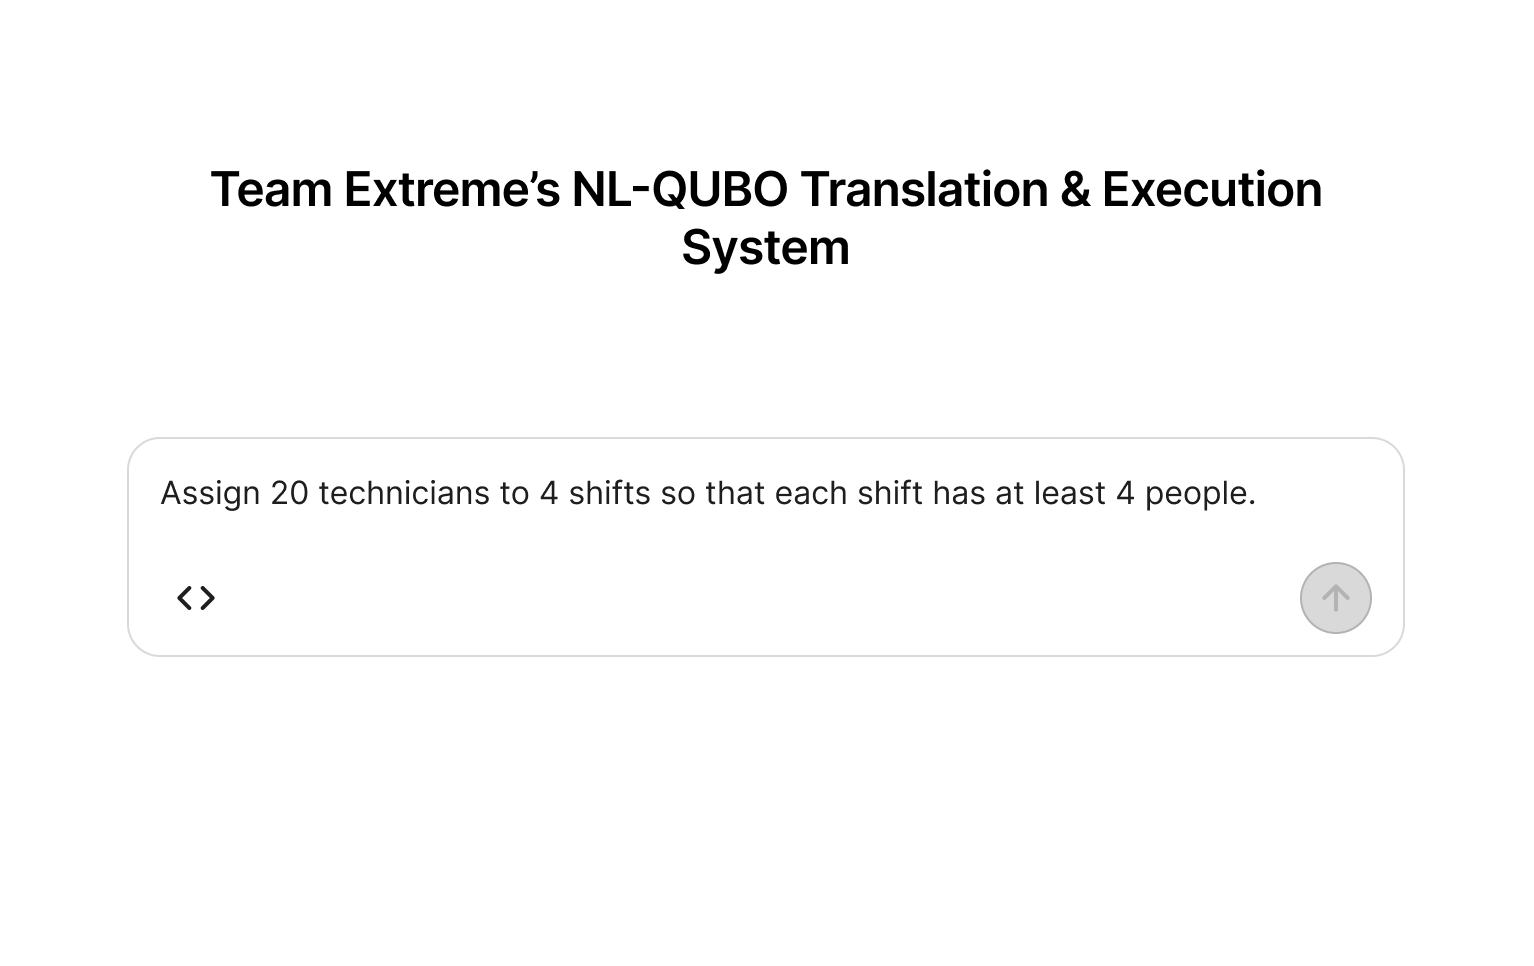
\includegraphics[width=0.9\linewidth]{png/UI1.png}}
    \caption{First UI prototype: prompt entry, translation status, QUBO
    summary, and fidelity score.}
    \label{fig:ui-frame1}
\end{figure}

\subsection{Frame 2: Local Solver Execution and Results}

Figure~\ref{fig:ui-frame2} shows the second screen of the prototype, which
appears after the user chooses to proceed to execution.  
The system runs the compiled QUBO on a local solver and reports the execution
status, the best objective value (for example, overtime hours), feasibility,
runtime, and a short solution preview that shows how technicians are assigned
to each shift.  
At the bottom, the UI asks whether the user would like to save logs and
metrics, preparing the transition to the logging and analysis features.

\begin{figure}[H]
    \centering
    \fbox{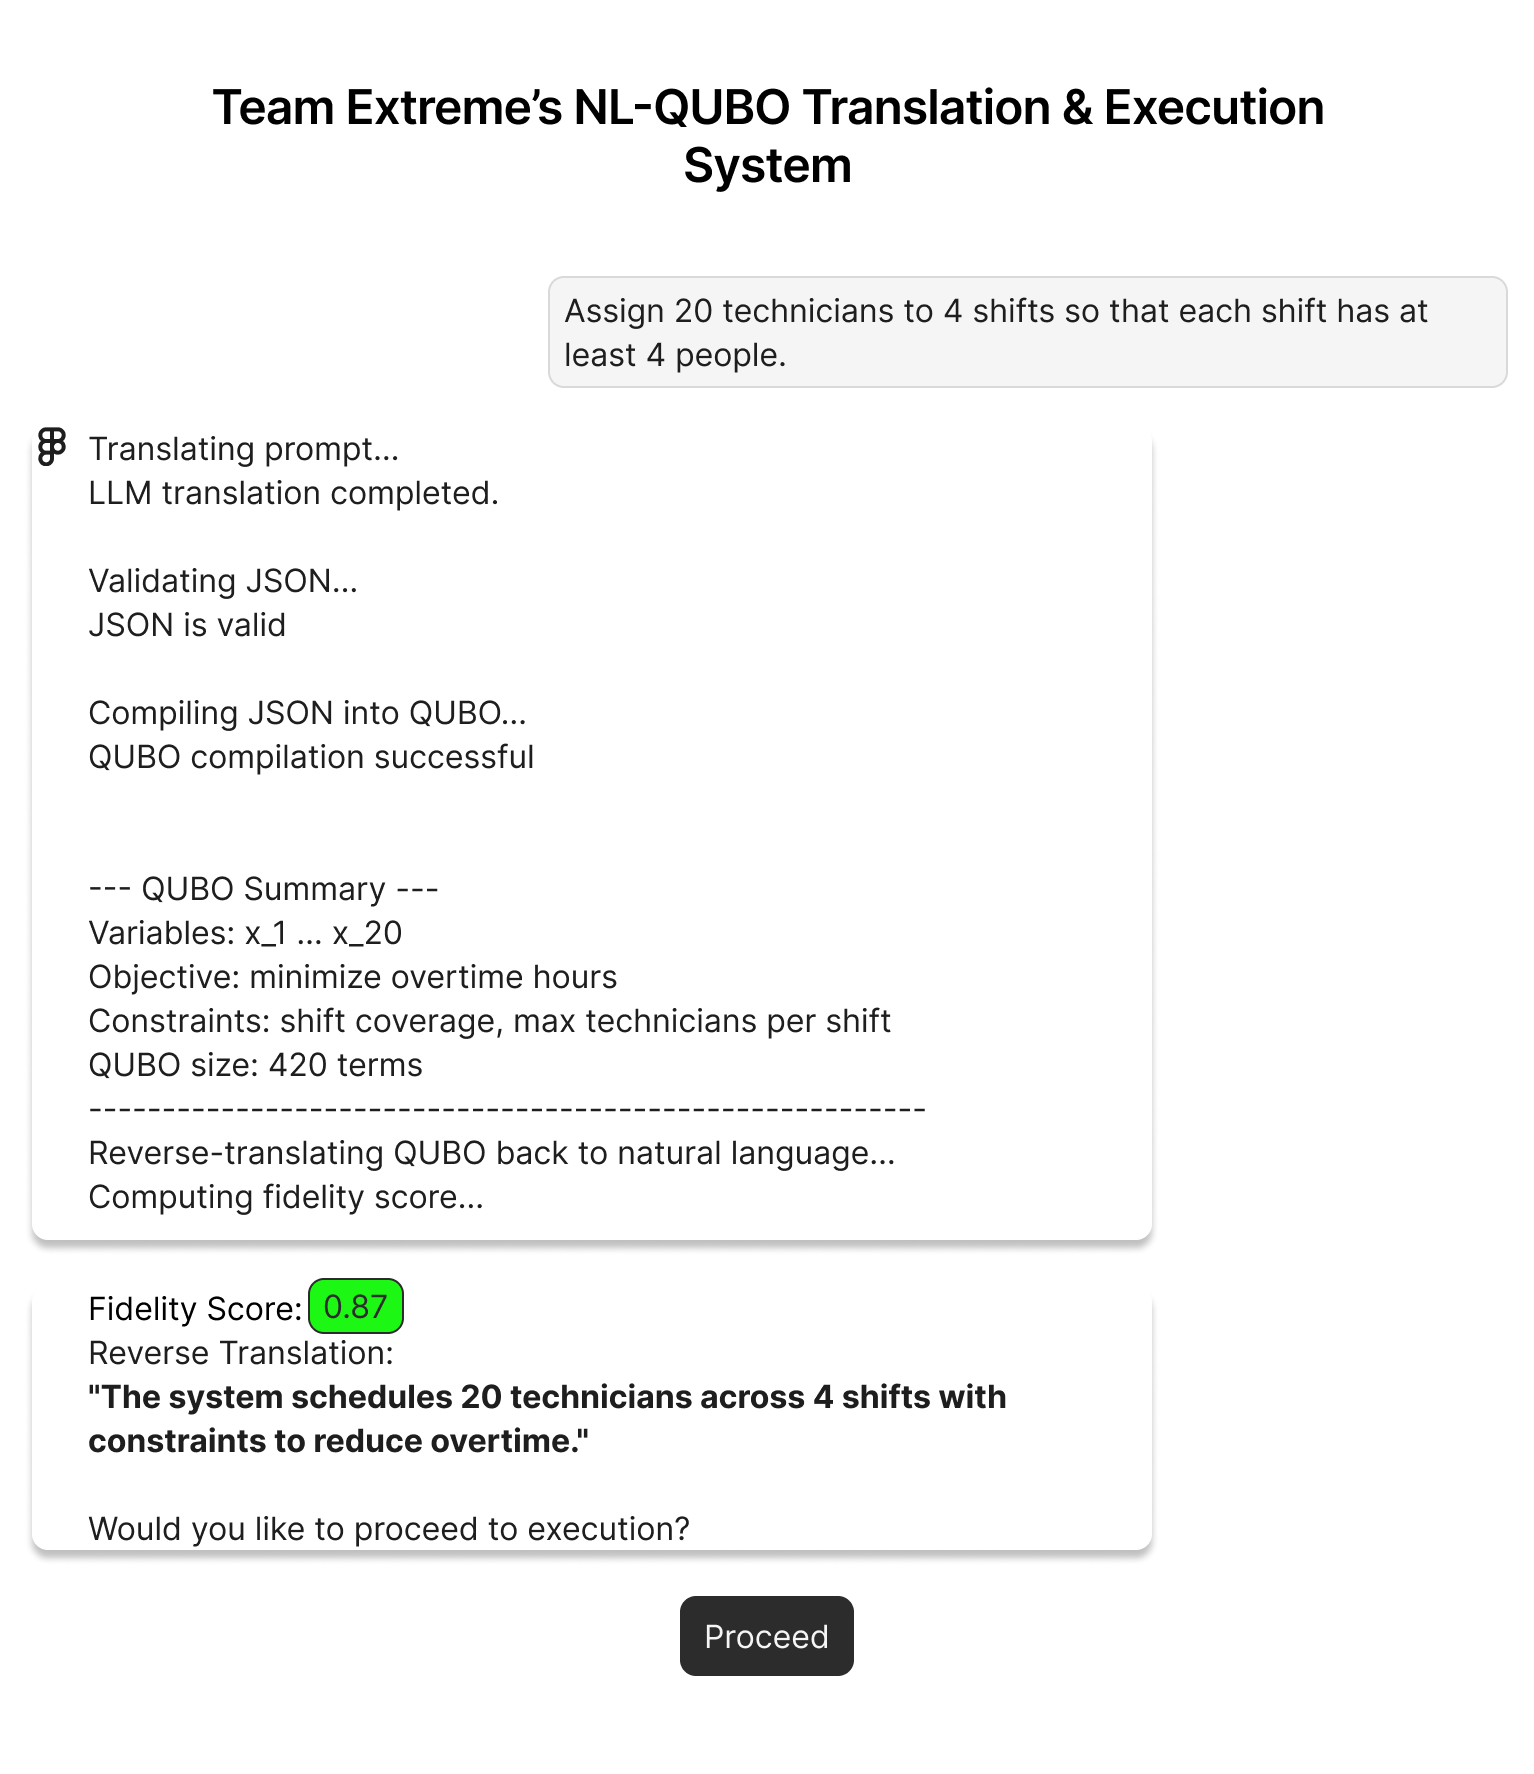
\includegraphics[width=0.9\linewidth]{png/UI2.png}}
    \caption{First UI prototype: local solver execution results and solution
    preview.}
    \label{fig:ui-frame2}
\end{figure}

\subsection{Frame 3: Logs and Metrics (Prototype Placeholder)}

Figure~\ref{fig:ui-frame3} represents the third frame of the first UI
prototype, focused on viewing and exporting logs and metrics from previous
runs.  
In the final system, this screen will allow users to review success rates,
latency, fidelity scores, and other performance metrics across multiple
experiments, as well as export CSV files or plots for further analysis.  
In this initial prototype, the layout is mainly illustrative and will be
refined once the logging back end and metrics pipeline are fully implemented.

\begin{figure}[H]
    \centering
    \fbox{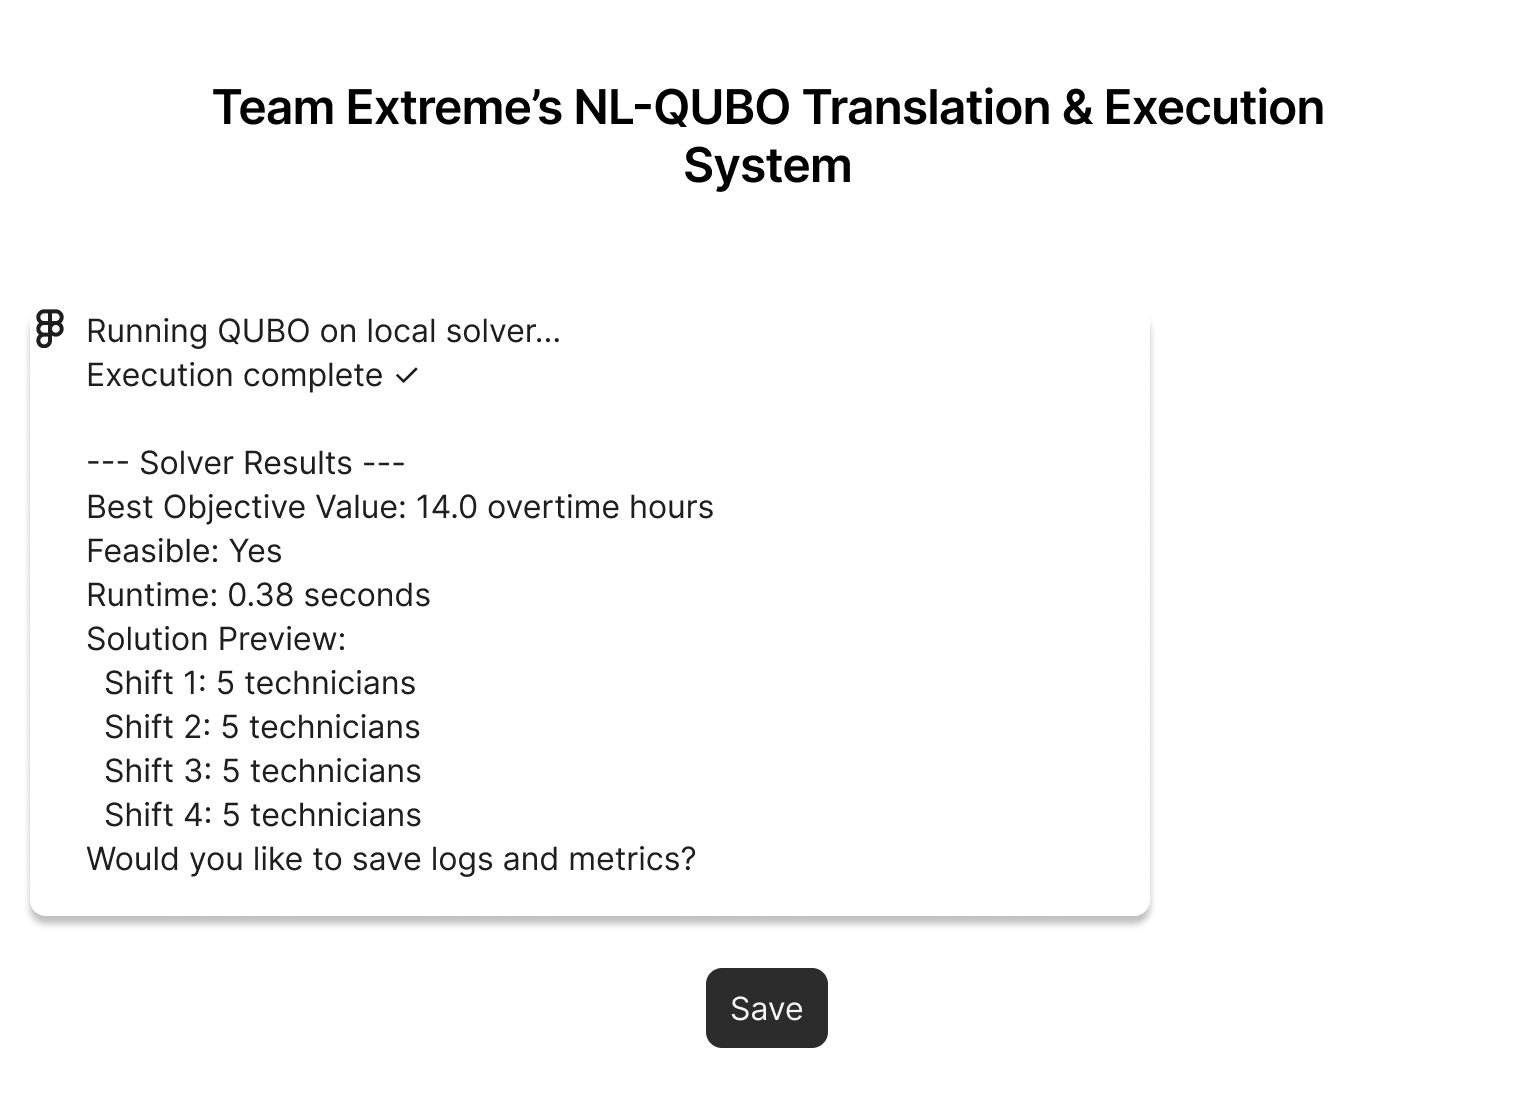
\includegraphics[width=0.9\linewidth]{png/UI3.png}}
    \caption{First UI prototype: conceptual layout for logs and metrics
    visualization and export.}
    \label{fig:ui-frame3}
\end{figure}
